\section{Utilização do projeto}

Para a Utilização do projeto basta a acessar a plataforma do github disponível em ``https://github.com/filipecancio/sbc-template'' e clicar na opção ``Use this template > Create New template'' como na figura~\ref{fig:image01}. A partir daqui preencher as novas informações necessárias para o novo projeto (figura~\ref{fig:image02}).

\begin{figure}[ht]
	\centering
	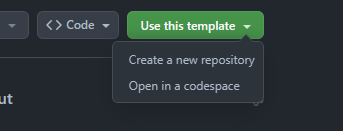
\includegraphics[width=.5\textwidth]{./images/image01.png}
	\caption{Adicionando um novo repositório a partir de um template}
	\label{fig:image01}
\end{figure}

\begin{figure}[ht]
	\centering
	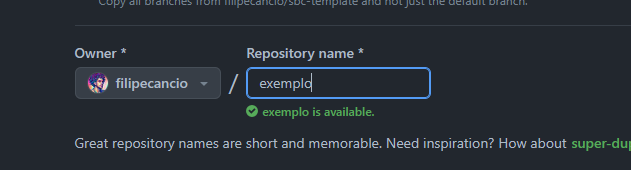
\includegraphics[width=.5\textwidth]{./images/image02.png}
	\caption{Adicionando informações
		de repositório}
	\label{fig:image02}
\end{figure}
Após criar um novo repositório, precisamos liberar o github para fazer mudanças automáticas no projeto. Para isso iremos em  ``settings > actions > general'' e na secao Workflow permissions colocar a opcao ``Read and write permissions'', depois clicar em ``save'' (figura~\ref{fig:image03}). Isso irá permitir que seja gerado o pdf automaticamente no repositorio futuramente.

\begin{figure}[ht]
	\centering
	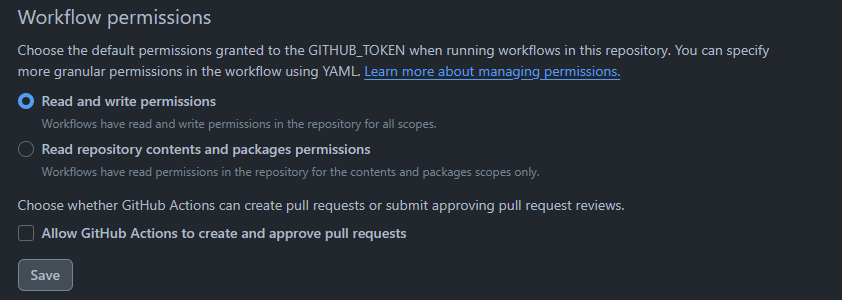
\includegraphics[width=.5\textwidth]{./images/image03.png}
	\caption{Alterando configurações do projeto}
	\label{fig:image03}
\end{figure}